\pagestyle{empty}
\chapter{Sistemas de Recomendaci�n Conversacionales}
\label{cap:sistemasRecomendacion}

\pagestyle{headings}


\begin{table*}[htbp]
\caption*{}
%\label{tabla:ejemploPeliculas}
\centering
%{\scriptsize
\begin{tabular}{p{4.0cm}p{7.0cm}}
 \hline
 T�tulo: & Enhancing the conversational process by using a logical closure operator in phenotypes implications\\
 Autores: & Fernando Benito-Picazo, Manuel Enciso, Carlos Rossi, Antonio Guevara\\
 Revista: & Mathematical Methods in the Applied Sciences, John Wiley \& Sons Ltd.\\
 Factor Impacto JCR: & 1,017. Posici�n 108 de 255 (Q2)\\
 A�o: & 2016\\
 Categor�a: & Mathematics, Applied\\
 Publicaci�n: & 16 febrero 2017\\
 DOI: & 10.1002/mma.4338\\
 \hline
\end{tabular}
%}
\end{table*}

\clearemptydoublepage

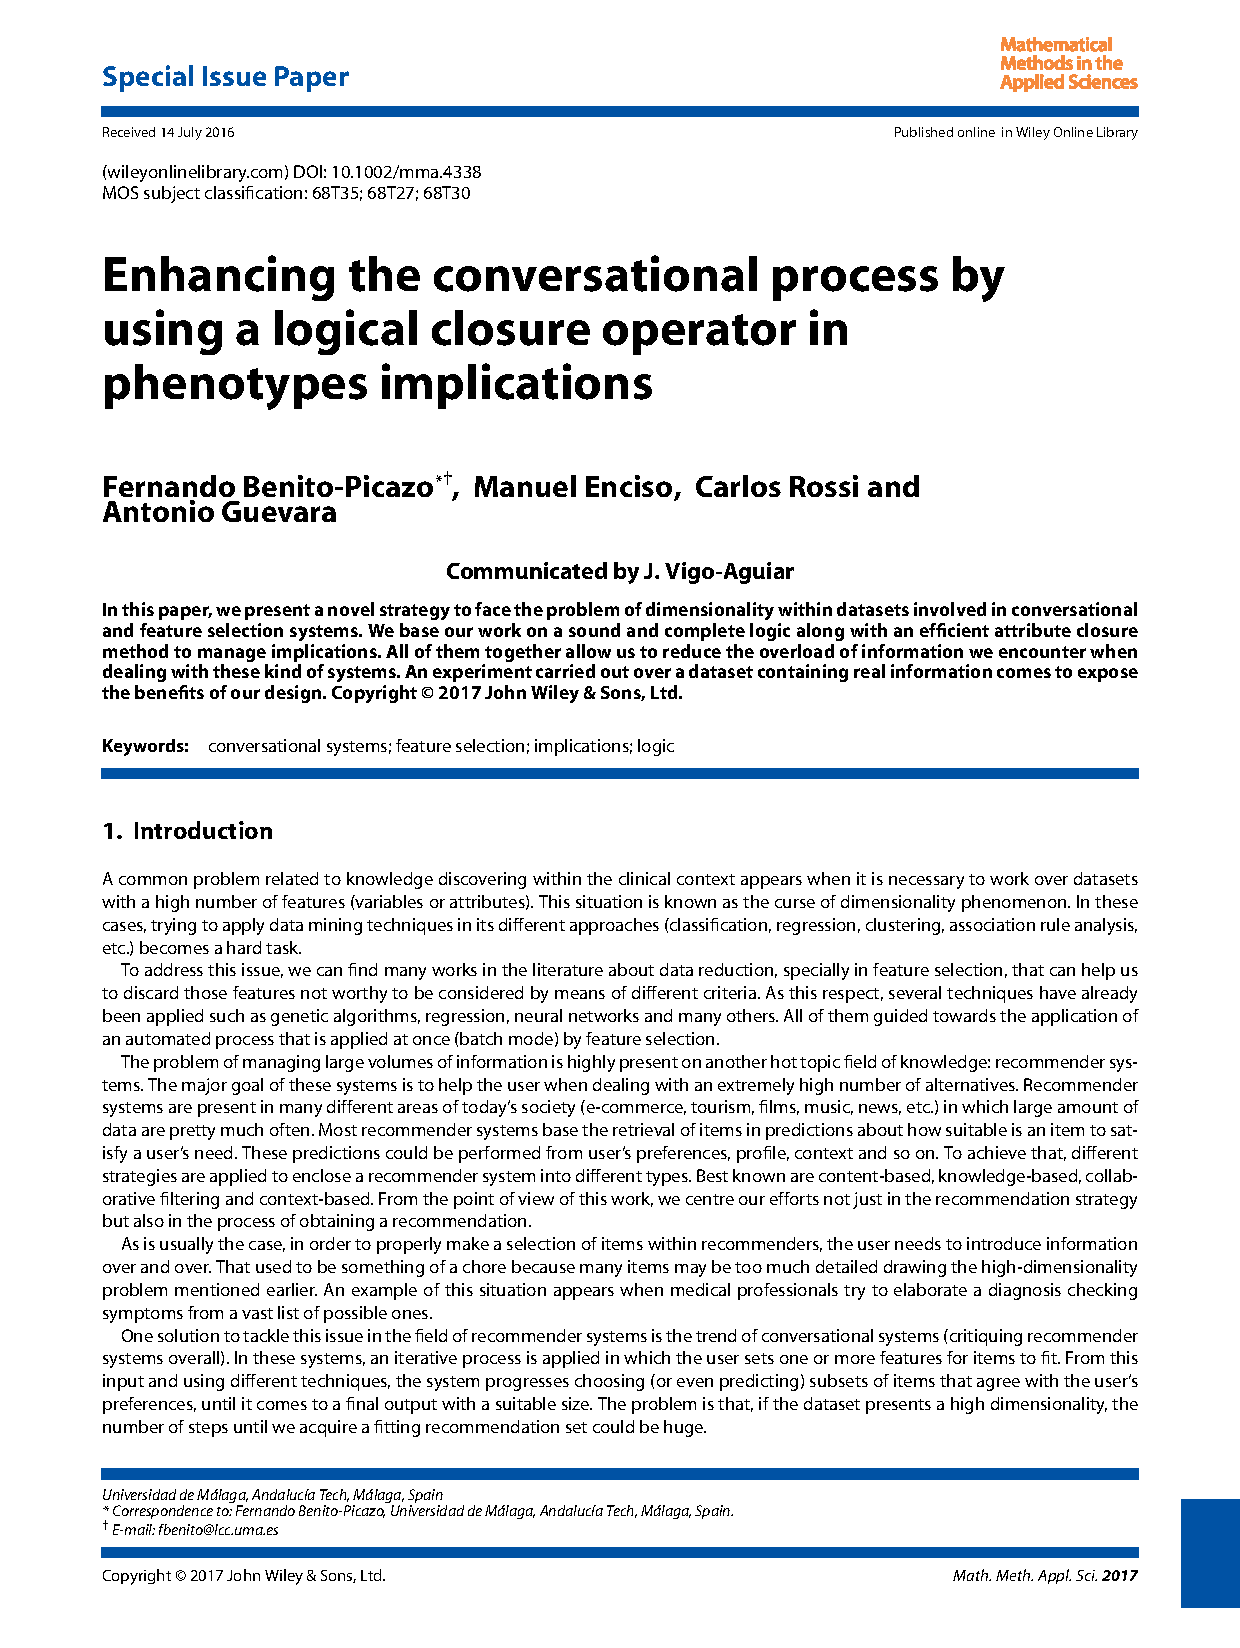
\includepdf[pages=-,scale=.9,pagecommand={}]{paperSistemaRecomendacionConversacional.pdf}

